% This file was created by tikzplotlib v0.9.4.
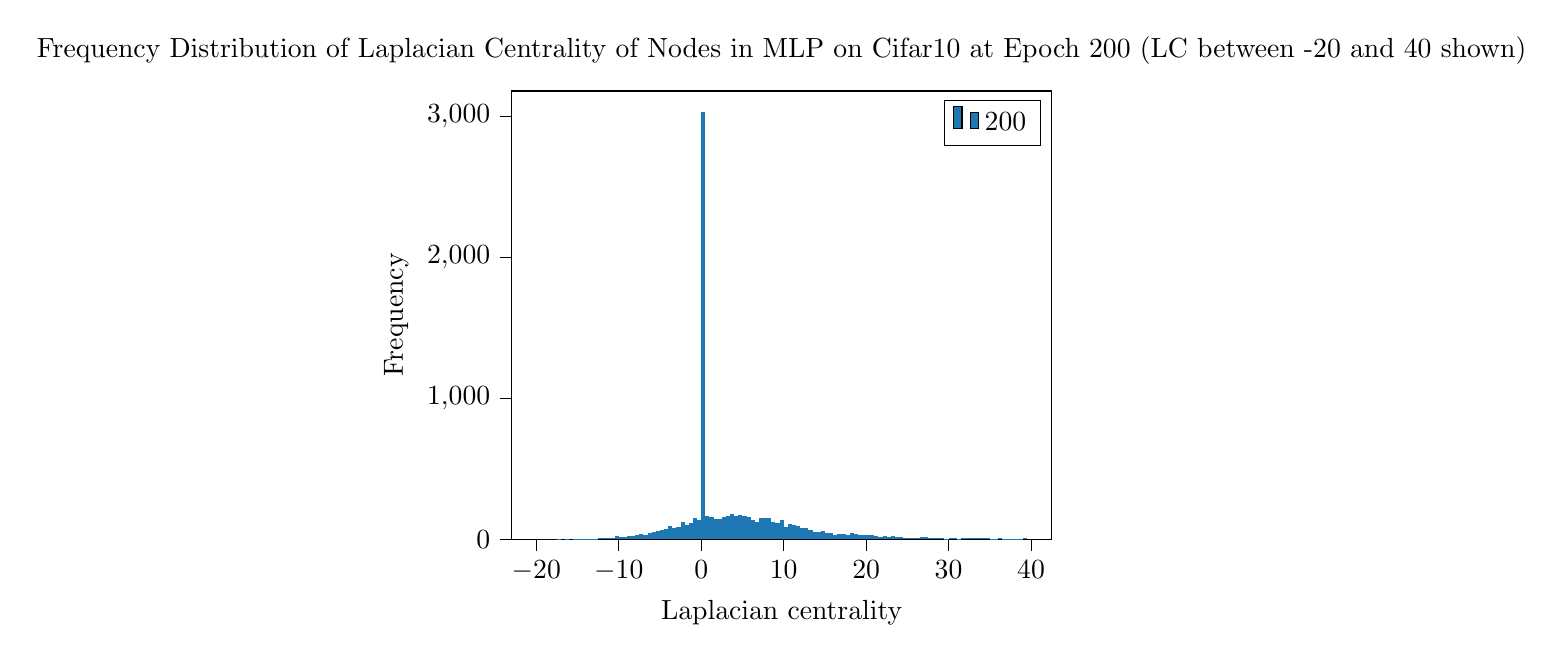
\begin{tikzpicture}

\definecolor{color0}{rgb}{0.12156862745098,0.466666666666667,0.705882352941177}

\begin{axis}[
tick align=outside,
tick pos=left,
title={Frequency Distribution of Laplacian Centrality of Nodes in MLP on Cifar10 at Epoch 200 (LC between -20 and 40 shown)},
x grid style={white!69.0196078431373!black},
xlabel={Laplacian centrality},
xmin=-22.975, xmax=42.475,
xtick style={color=black},
y grid style={white!69.0196078431373!black},
ylabel={Frequency},
ymin=0, ymax=3180.45,
ytick style={color=black}
]
\draw[draw=none,fill=color0] (axis cs:-20,0) rectangle (axis cs:-19.5,0);
\addlegendimage{ybar,ybar legend,draw=none,fill=color0};
\addlegendentry{200}

\draw[draw=none,fill=color0] (axis cs:-19.5,0) rectangle (axis cs:-19,0);
\draw[draw=none,fill=color0] (axis cs:-19,0) rectangle (axis cs:-18.5,0);
\draw[draw=none,fill=color0] (axis cs:-18.5,0) rectangle (axis cs:-18,0);
\draw[draw=none,fill=color0] (axis cs:-18,0) rectangle (axis cs:-17.5,0);
\draw[draw=none,fill=color0] (axis cs:-17.5,0) rectangle (axis cs:-17,1);
\draw[draw=none,fill=color0] (axis cs:-17,0) rectangle (axis cs:-16.5,0);
\draw[draw=none,fill=color0] (axis cs:-16.5,0) rectangle (axis cs:-16,2);
\draw[draw=none,fill=color0] (axis cs:-16,0) rectangle (axis cs:-15.5,0);
\draw[draw=none,fill=color0] (axis cs:-15.5,0) rectangle (axis cs:-15,2);
\draw[draw=none,fill=color0] (axis cs:-15,0) rectangle (axis cs:-14.5,4);
\draw[draw=none,fill=color0] (axis cs:-14.5,0) rectangle (axis cs:-14,4);
\draw[draw=none,fill=color0] (axis cs:-14,0) rectangle (axis cs:-13.5,3);
\draw[draw=none,fill=color0] (axis cs:-13.5,0) rectangle (axis cs:-13,2);
\draw[draw=none,fill=color0] (axis cs:-13,0) rectangle (axis cs:-12.5,4);
\draw[draw=none,fill=color0] (axis cs:-12.5,0) rectangle (axis cs:-12,7);
\draw[draw=none,fill=color0] (axis cs:-12,0) rectangle (axis cs:-11.5,10);
\draw[draw=none,fill=color0] (axis cs:-11.5,0) rectangle (axis cs:-11,9);
\draw[draw=none,fill=color0] (axis cs:-11,0) rectangle (axis cs:-10.5,11);
\draw[draw=none,fill=color0] (axis cs:-10.5,0) rectangle (axis cs:-10,22);
\draw[draw=none,fill=color0] (axis cs:-10,0) rectangle (axis cs:-9.5,16);
\draw[draw=none,fill=color0] (axis cs:-9.5,0) rectangle (axis cs:-9,19);
\draw[draw=none,fill=color0] (axis cs:-9,0) rectangle (axis cs:-8.5,25);
\draw[draw=none,fill=color0] (axis cs:-8.5,0) rectangle (axis cs:-8,23);
\draw[draw=none,fill=color0] (axis cs:-8,0) rectangle (axis cs:-7.5,28);
\draw[draw=none,fill=color0] (axis cs:-7.5,0) rectangle (axis cs:-7,39);
\draw[draw=none,fill=color0] (axis cs:-7,0) rectangle (axis cs:-6.5,31);
\draw[draw=none,fill=color0] (axis cs:-6.5,0) rectangle (axis cs:-6,43);
\draw[draw=none,fill=color0] (axis cs:-6,0) rectangle (axis cs:-5.5,54);
\draw[draw=none,fill=color0] (axis cs:-5.5,0) rectangle (axis cs:-5,62);
\draw[draw=none,fill=color0] (axis cs:-5,0) rectangle (axis cs:-4.5,67);
\draw[draw=none,fill=color0] (axis cs:-4.5,0) rectangle (axis cs:-4,74);
\draw[draw=none,fill=color0] (axis cs:-4,0) rectangle (axis cs:-3.5,92);
\draw[draw=none,fill=color0] (axis cs:-3.5,0) rectangle (axis cs:-3,81);
\draw[draw=none,fill=color0] (axis cs:-3,0) rectangle (axis cs:-2.5,89);
\draw[draw=none,fill=color0] (axis cs:-2.5,0) rectangle (axis cs:-2,120);
\draw[draw=none,fill=color0] (axis cs:-2,0) rectangle (axis cs:-1.5,104);
\draw[draw=none,fill=color0] (axis cs:-1.5,0) rectangle (axis cs:-1,117);
\draw[draw=none,fill=color0] (axis cs:-1,0) rectangle (axis cs:-0.5,149);
\draw[draw=none,fill=color0] (axis cs:-0.5,0) rectangle (axis cs:0,140);
\draw[draw=none,fill=color0] (axis cs:0,0) rectangle (axis cs:0.5,3029);
\draw[draw=none,fill=color0] (axis cs:0.5,0) rectangle (axis cs:1,162);
\draw[draw=none,fill=color0] (axis cs:1,0) rectangle (axis cs:1.5,159);
\draw[draw=none,fill=color0] (axis cs:1.5,0) rectangle (axis cs:2,146);
\draw[draw=none,fill=color0] (axis cs:2,0) rectangle (axis cs:2.5,142);
\draw[draw=none,fill=color0] (axis cs:2.5,0) rectangle (axis cs:3,155);
\draw[draw=none,fill=color0] (axis cs:3,0) rectangle (axis cs:3.5,162);
\draw[draw=none,fill=color0] (axis cs:3.5,0) rectangle (axis cs:4,177);
\draw[draw=none,fill=color0] (axis cs:4,0) rectangle (axis cs:4.5,165);
\draw[draw=none,fill=color0] (axis cs:4.5,0) rectangle (axis cs:5,170);
\draw[draw=none,fill=color0] (axis cs:5,0) rectangle (axis cs:5.5,167);
\draw[draw=none,fill=color0] (axis cs:5.5,0) rectangle (axis cs:6,158);
\draw[draw=none,fill=color0] (axis cs:6,0) rectangle (axis cs:6.5,136);
\draw[draw=none,fill=color0] (axis cs:6.5,0) rectangle (axis cs:7,124);
\draw[draw=none,fill=color0] (axis cs:7,0) rectangle (axis cs:7.5,153);
\draw[draw=none,fill=color0] (axis cs:7.5,0) rectangle (axis cs:8,153);
\draw[draw=none,fill=color0] (axis cs:8,0) rectangle (axis cs:8.5,148);
\draw[draw=none,fill=color0] (axis cs:8.5,0) rectangle (axis cs:9,123);
\draw[draw=none,fill=color0] (axis cs:9,0) rectangle (axis cs:9.5,114);
\draw[draw=none,fill=color0] (axis cs:9.5,0) rectangle (axis cs:10,137);
\draw[draw=none,fill=color0] (axis cs:10,0) rectangle (axis cs:10.5,86);
\draw[draw=none,fill=color0] (axis cs:10.5,0) rectangle (axis cs:11,106);
\draw[draw=none,fill=color0] (axis cs:11,0) rectangle (axis cs:11.5,99);
\draw[draw=none,fill=color0] (axis cs:11.5,0) rectangle (axis cs:12,96);
\draw[draw=none,fill=color0] (axis cs:12,0) rectangle (axis cs:12.5,82);
\draw[draw=none,fill=color0] (axis cs:12.5,0) rectangle (axis cs:13,79);
\draw[draw=none,fill=color0] (axis cs:13,0) rectangle (axis cs:13.5,67);
\draw[draw=none,fill=color0] (axis cs:13.5,0) rectangle (axis cs:14,53);
\draw[draw=none,fill=color0] (axis cs:14,0) rectangle (axis cs:14.5,51);
\draw[draw=none,fill=color0] (axis cs:14.5,0) rectangle (axis cs:15,60);
\draw[draw=none,fill=color0] (axis cs:15,0) rectangle (axis cs:15.5,43);
\draw[draw=none,fill=color0] (axis cs:15.5,0) rectangle (axis cs:16,43);
\draw[draw=none,fill=color0] (axis cs:16,0) rectangle (axis cs:16.5,29);
\draw[draw=none,fill=color0] (axis cs:16.5,0) rectangle (axis cs:17,35);
\draw[draw=none,fill=color0] (axis cs:17,0) rectangle (axis cs:17.5,35);
\draw[draw=none,fill=color0] (axis cs:17.5,0) rectangle (axis cs:18,32);
\draw[draw=none,fill=color0] (axis cs:18,0) rectangle (axis cs:18.5,45);
\draw[draw=none,fill=color0] (axis cs:18.5,0) rectangle (axis cs:19,40);
\draw[draw=none,fill=color0] (axis cs:19,0) rectangle (axis cs:19.5,31);
\draw[draw=none,fill=color0] (axis cs:19.5,0) rectangle (axis cs:20,31);
\draw[draw=none,fill=color0] (axis cs:20,0) rectangle (axis cs:20.5,27);
\draw[draw=none,fill=color0] (axis cs:20.5,0) rectangle (axis cs:21,32);
\draw[draw=none,fill=color0] (axis cs:21,0) rectangle (axis cs:21.5,24);
\draw[draw=none,fill=color0] (axis cs:21.5,0) rectangle (axis cs:22,19);
\draw[draw=none,fill=color0] (axis cs:22,0) rectangle (axis cs:22.5,20);
\draw[draw=none,fill=color0] (axis cs:22.5,0) rectangle (axis cs:23,16);
\draw[draw=none,fill=color0] (axis cs:23,0) rectangle (axis cs:23.5,20);
\draw[draw=none,fill=color0] (axis cs:23.5,0) rectangle (axis cs:24,14);
\draw[draw=none,fill=color0] (axis cs:24,0) rectangle (axis cs:24.5,19);
\draw[draw=none,fill=color0] (axis cs:24.5,0) rectangle (axis cs:25,11);
\draw[draw=none,fill=color0] (axis cs:25,0) rectangle (axis cs:25.5,6);
\draw[draw=none,fill=color0] (axis cs:25.5,0) rectangle (axis cs:26,10);
\draw[draw=none,fill=color0] (axis cs:26,0) rectangle (axis cs:26.5,11);
\draw[draw=none,fill=color0] (axis cs:26.5,0) rectangle (axis cs:27,13);
\draw[draw=none,fill=color0] (axis cs:27,0) rectangle (axis cs:27.5,13);
\draw[draw=none,fill=color0] (axis cs:27.5,0) rectangle (axis cs:28,9);
\draw[draw=none,fill=color0] (axis cs:28,0) rectangle (axis cs:28.5,8);
\draw[draw=none,fill=color0] (axis cs:28.5,0) rectangle (axis cs:29,9);
\draw[draw=none,fill=color0] (axis cs:29,0) rectangle (axis cs:29.5,7);
\draw[draw=none,fill=color0] (axis cs:29.5,0) rectangle (axis cs:30,5);
\draw[draw=none,fill=color0] (axis cs:30,0) rectangle (axis cs:30.5,8);
\draw[draw=none,fill=color0] (axis cs:30.5,0) rectangle (axis cs:31,12);
\draw[draw=none,fill=color0] (axis cs:31,0) rectangle (axis cs:31.5,5);
\draw[draw=none,fill=color0] (axis cs:31.5,0) rectangle (axis cs:32,7);
\draw[draw=none,fill=color0] (axis cs:32,0) rectangle (axis cs:32.5,6);
\draw[draw=none,fill=color0] (axis cs:32.5,0) rectangle (axis cs:33,11);
\draw[draw=none,fill=color0] (axis cs:33,0) rectangle (axis cs:33.5,7);
\draw[draw=none,fill=color0] (axis cs:33.5,0) rectangle (axis cs:34,6);
\draw[draw=none,fill=color0] (axis cs:34,0) rectangle (axis cs:34.5,8);
\draw[draw=none,fill=color0] (axis cs:34.5,0) rectangle (axis cs:35,6);
\draw[draw=none,fill=color0] (axis cs:35,0) rectangle (axis cs:35.5,4);
\draw[draw=none,fill=color0] (axis cs:35.5,0) rectangle (axis cs:36,4);
\draw[draw=none,fill=color0] (axis cs:36,0) rectangle (axis cs:36.5,7);
\draw[draw=none,fill=color0] (axis cs:36.5,0) rectangle (axis cs:37,2);
\draw[draw=none,fill=color0] (axis cs:37,0) rectangle (axis cs:37.5,3);
\draw[draw=none,fill=color0] (axis cs:37.5,0) rectangle (axis cs:38,1);
\draw[draw=none,fill=color0] (axis cs:38,0) rectangle (axis cs:38.5,5);
\draw[draw=none,fill=color0] (axis cs:38.5,0) rectangle (axis cs:39,4);
\draw[draw=none,fill=color0] (axis cs:39,0) rectangle (axis cs:39.5,6);
\end{axis}

\end{tikzpicture}
